%%\documentclass[pdflatex,sn-nature]{sn-jnl}% Style for submissions to Nature Portfolio journals
%%\documentclass[pdflatex,sn-basic]{sn-jnl}% Basic Springer Nature Reference Style/Chemistry Reference Style
\documentclass[pdflatex,sn-mathphys-num]{sn-jnl}% Math and Physical Sciences Numbered Reference Style 
%%\documentclass[pdflatex,sn-mathphys-ay]{sn-jnl}% Math and Physical Sciences Author Year Reference Style
%%\documentclass[pdflatex,sn-aps]{sn-jnl}% American Physical Society (APS) Reference Style
%%\documentclass[pdflatex,sn-vancouver,Numbered]{sn-jnl}% Vancouver Reference Style
%%\documentclass[pdflatex,sn-apa]{sn-jnl}% APA Reference Style 
%%\documentclass[pdflatex,sn-chicago]{sn-jnl}% Chicago-based Humanities Reference Style

\usepackage{graphicx}%
\usepackage{multirow}%
\usepackage{amsmath,amssymb,amsfonts}%
\usepackage{amsthm}%
\usepackage{mathrsfs}%
\usepackage[title]{appendix}%
\usepackage{xcolor}%
\usepackage{textcomp}%
\usepackage{manyfoot}%
\usepackage{booktabs}%
\usepackage{algorithm}%
\usepackage{algorithmicx}%
\usepackage{algpseudocode}%
\usepackage{listings}%
\theoremstyle{thmstyleone}%
\newtheorem{theorem}{Theorem}%
\newtheorem{proposition}[theorem]{Proposition}%
\theoremstyle{thmstyletwo}%
\newtheorem{example}{Example}%
\newtheorem{remark}{Remark}%
\theoremstyle{thmstylethree}%
\newtheorem{definition}{Definition}%
\raggedbottom



\begin{document}

\title[Article Title]{DAP-PIR: Efficient Genetic Association Analysis through Pseudo Importance Resampling}

\author[1]{\fnm{Bo} \sur{Wang}}\email{wnbo@umich.edu}

\author*[1]{\fnm{Xiaoquan} \sur{Wen}}\email{xwen@umich.edu}

\affil[1]{\orgdiv{Department of Biostatistics}, \orgname{University of Michigan}, \orgaddress{\city{Ann Arbor}, \state{MI} \postcode{48109}, \country{USA}}}

\abstract{In genome-wide association studies (GWAS), identifying causal variants from a vast number of genetic variants is challenging. This paper presents DAP-PIR, a method combining Deterministic Approximation of Posteriors (DAP) with Pseudo-Importance Resampling (PIR), to enhance computational efficiency and improve the accuracy of fine-mapping in genetic studies. By selecting a limited number of high-probability models, DAP-PIR effectively narrows down the candidate models, maintaining accuracy in posterior estimation while reducing computational costs. Simulations and real data analyses show the superiority of DAP-PIR over existing methods, including SuSiE, particularly in managing high-dimensional genetic data.}


\keywords{Genetic fine mapping, variable selection, importance sampling, variational inference}

\maketitle



\section{Introduction}\label{sec1}
Genome-wide association studies (GWAS) have successfully uncovered thousands of genetic variants associated with complex traits and diseases \cite{visscher201710}. However, due to the intricate linkage disequilibrium (LD) structure in the human genome, many variants identified in GWAS are merely correlated with true causal variants rather than causative themselves \cite{ardlie2002patterns}. Fine mapping analysis is therefore essential to refine these associations and identify specific genetic variants likely to be causal \cite{spain2015strategies, schaid2018genome}.

To address this challenge, Bayesian variable selection regression (BVSR) methods are widely employed to account for the uncertainty in identifying candidate causal variants. Traditional methods like CAVIAR rely on exhaustive searches \cite{hormozdiari2014identifying}, while DAP-G employs a boosting approach to prioritize variants, which, although effective, can sometimes be slow in practice \cite{wen2016efficient, lee2018bayesian}. Alternatively, the SuSiE method offers an efficient, variational approach to prioritize SNPs based on posterior inclusion probabilities (PIP) \cite{wang2020simple}. However, SuSiE can occasionally experience accuracy issues with PIP, particularly in complex LD structures.

Here, we propose DAP-PIR, which combines the strengths of both DAP and SuSiE to achieve efficient and accurate deterministic approximation of posteriors. By leveraging SuSiE's variational approximation results, DAP-PIR efficiently prioritizes models for deterministic posterior estimation. This approach ensures computational efficiency while providing a robust solution to fine mapping challenges in GWAS. Through both simulations and real data applications, we demonstrate DAP-PIR’s advantages over existing methods in terms of both speed and accuracy, making it an effective tool for fine mapping causal variants in GWAS.



\section{Results}\label{sec2}
\subsection{Overview of the DAP-PIR algorithm}\label{subsec1}
The DAP-PIR algorithm uses two steps to efficiently approximate the posteiror distributions both at the variant-level and cluster-level. In the first step, the algorithm utilizes the variational approximation of the posterior distribution in a lower dimensional space as the proposal distribution in the importance sampling. Then, the algorithm employs the pseudo importance resampling (PIR) to further reduce the sample space and avoiding the need to draw random samples, instead focus on the high-probability regions. In the second step, the algorithm conduct the deterministic approximation of posteriors (DAP) by calculating the posterior inclusion probabilities (PIPs) for each high-probability model obtained in the first step by marginalizing over the priror. The DAP-PIR algorithm outputs the PIP of each variant by marginalizing the posterior model probability, and also provides level-$\rho$ credible sets, which is a subset of variants that has a specific probability of containing at least one causal variants.





\subsection{Simulation studies}\label{subsec3}
\subsubsection*{Accuracy of the DAP-PIR algorithm}
To demonstrate the accuracy and efficiency of the DAP-PIR algorithm, we first compare its posterior approxmiations to those obtained through exact calculations. We simulate genotypes from a standard normal distribution and focus on a scenariow with $p=10$ \textit{cis}-SNPs to reduce the computational burden of exact posterior calculations. We randomly select one to five variants as causal and generate phenotypes after adding random noise. For each scenario, we conduct 1,000 simulations. The approxiamtions of posteriors obtained via the DAP-PIR algorithm are then compared with the exact posterior calculations.

Using a dataset of 5,000 simulations, we evaluate the performance of the DAP-PIR algorithm alongside exact posteiror calculations and results from the DAP-G algorithm, employing the same prior specifications for all methods. The SuSiE algorithm is also included to assess its posterior approximations. For the DAP-PIR algorithm, we set the threshold value $\lambda=10^{-6}$.

We begin by exmaining the ratio of the estimated normalizing constant $C^*$ from the DAP-PIR and DAP-G algorithms to the true normalizing constant $C^*$, derived from exact calculations. For the $C^*/C$, a value close to 1 means a better model space exploration. The results, presented in Figures \ref{fig1}-\ref{fig5}, reveal that the DAP-PIR algorithm achieves a high $C^*/C$ raio across various numbers of causal effects. This indicates that the DAP-PIR algorithm efficiently explores high-probability model spaces and provides a more accurate estimate of the normalizing constant compared to the DAP-G algorithm.

Additionally, the Root Mean Squared Error (RMSE) of the PIPs from the DAP-PIR algorithm is smaller than that of both the DAP-G and SuSiE algorithms, demonstrating better posterior approxiamtion. Calibration plots (Figures \ref{fig11}-\ref{fig51}) further confirm that the DAP-PIR algorithm yields more accurate PIP estimates for each vairant than the other methods.

Notably, the DAP-PIR algorithm explores a significantly smaller number of models, with the median number of explored models much lower than the $2^{10}=1,024$ models required for exact calculations. This demonstrates that by focusing on high-probability regions of the model space, the algorithm achieves accurate posterior approximations while remaining computationally efficient, particularly as $p$ increases.


\begin{table}[h]
    \caption{Performance comparison of different methods at propensity threshold $10^{-6}$.}\label{tab:comparison}
    \begin{tabular*}{\textwidth}{@{\extracolsep\fill}c*{7}{c}}
    \toprule
    & \multicolumn{2}{@{}c@{}}{Mean of $C^*/C$} & \multicolumn{2}{@{}c@{}}{Median Model Numbers} & \multicolumn{3}{@{}c@{}}{RMSE of approximate PIP} \\
    \cmidrule(r){2-3} \cmidrule(r){4-5} \cmidrule(r){6-8}
    $S$ & DAP-G & DAP-PIR & DAP-G & DAP-PIR & DAP-G & DAP-PIR & SuSiE \\
    \midrule
    1 & $0.922$ & $0.999$ & 13 & 114 & $8.05 \times 10^{-3}$ & $3.93 \times 10^{-5}$ & $1.42 \times 10^{-1}$ \\
    2 & $0.913$ & $0.999$ & 14 & 101 & $9.01 \times 10^{-3}$ & $4.44 \times 10^{-5}$ & $1.12 \times 10^{-1}$ \\
    3 & $0.915$ & $0.999$ & 14 & 91 & $9.71 \times 10^{-3}$ & $7.14 \times 10^{-5}$ & $8.88 \times 10^{-2}$ \\
    4 & $0.922$ & $0.999$ & 15 & 81 & $9.40 \times 10^{-3}$ & $1.11 \times 10^{-4}$ & $7.57 \times 10^{-2}$ \\
    5 & $0.928$ & $0.998$ & 16 & 74 & $9.87 \times 10^{-3}$ & $5.45 \times 10^{-4}$ & $6.02 \times 10^{-2}$ \\
    \botrule
    \end{tabular*}
\end{table}




\subsubsection*{Power comparions of fine mapping algorithms}
We conduct several simulation studies to show the accuracy and efficiency of the DAP-PIR algorithm. Comparing the (1) power; (2) coverage; (3) PIP calibration; (4) computational efficiency among fine mapping methods.



\subsection{Real data results}\label{subsec4}
We analyze some real data using various fine mapping methods.

\section{Discussion}\label{sec3}



\newpage
\section{Methods}\label{sec4}
\subsection{Bayesian variable selection model}
We consider the context of association analysis for a single quantitative trait. Let $\mathbf{y}=\left(y_1,y_2,\cdots,y_n\right)^T$ denote an $n$-dimensional vector representing the trait of interest, $\mathbf{G} = \left(\mathbf{g}_1,\mathbf{g}_2,\cdots,\mathbf{g}_p\right)$ represent an $n \times p$ genotype matrix, where each column $\mathbf{g}_j$ is an $n$-dimensional vector of genotypes for the $j$-th variant. We assume that $\mathbf{y}$ and the columns of $\mathbf{G}$ are centered to have a mean of zero to avoid the need for an intercept term. The model is then defined as:
\begin{equation}
    \mathbf{y} = \sum_{j=1}^{p} \beta_j \mathbf{g}_j  + \mathbf{e}, \; \mathbf{e} \sim N_n\left(0, \tau^{-1}I_n\right),
\end{equation}
where $\beta_j$ denotes the genetic effect of the $j$-th variant, and $\tau$ represents the precision. The goal of GWAS fine mapping is to prioritize causal variants rather than estimate their effect sizes, therefore we introduce an inclusion indicator $\gamma_j = I(\beta_j \neq 0)$ for each variant, where $\gamma_j=1$ indicates that the $j$-th variant is causal. The primary aim is infer the posterior distribution of the causal status vector: $\boldsymbol{\gamma} = \left(\gamma_1,\gamma_2,\cdots,\gamma_p\right)^T$. While evaluating each possible model configuration $\boldsymbol{\gamma}$ is straightforward as it only requires integrating out $\beta_j$'s and $\tau$, summing over all $2^p$ model configurations becomes computationally intractable as $p$ increases. This makes traditional Markov Chain Monte Carlo (MCMC) methods inefficient for fine mapping tasks involving even a moderate number of variants. Therefore, we utilize the efficient pseudo importance resampling method to explore the model space and approximate the posterior distribution of $\boldsymbol{\gamma}$.



\subsection{Pseudo importance resampling}
For a discrete random variable $\mathbf{X}$ with target distribution $p\left(\mathbf{x}\right)$, the objective is to approxiamte the expectation $\mathbb{E}_{p}[f\left( \mathbf{X} \right)]$ for a function $f\left(\mathbf{x}\right) = \mathbf{x}$. Due to the high-dimensional sample space, exact computation is impractical. We employ Importance Sampling to estimate this expectation by sampling from a proposal distribution $q\left(\mathbf{x}\right)$ and assigning importance weights $w\left( \mathbf{x}^{i} \right) = p\left(\mathbf{x}^{i}\right)/q\left(\mathbf{x}^{i}\right)$ for samples $\mathbf{x}^i \sim q\left(\mathbf{x}\right)$. The IS estimate is:
\begin{equation}
    \tilde{\boldsymbol{\mu}}_{\operatorname{IS}} =  \frac{\sum_{i=1}^{n}w\left( \mathbf{x}^{i} \right) f\left( \mathbf{x}^{i} \right)}{\sum_{i=1}^n w\left( \mathbf{x}^{i} \right)}.
\end{equation}
To obtain a reliable estimate, $q\left(\mathbf{x}\right)$ should closely approximate $p\left(\mathbf{x}\right)$, particularly in regions where $f\left(\mathbf{x}\right)p\left(\mathbf{x}\right)$ has significant values.

We use Variational Approximation (VA) to construct an effective proposal distribution by minimizing the Kullback-Leibler (KL) divergence between $p\left(\mathbf{x}\right)$ to $q\left(\mathbf{x}\right)$. VA provides a tractable approxiamtion, balancing efficiency and accuracy. The Variational Importance Sampling (VIS) method integrates VA with IS, leveraging VA's computational efficiency while reducing bias through IS.

\begin{algorithm}
    \caption{Variational Importance Sampling (VIS)}
    \label{alg:variational_is}
    \begin{enumerate}
        \item Target distribution: derive the analytical expression of \(p'(\mathbf{x})\) up to a normalizing constant.
        \item Proposal distribution: obtain the variational approximation \( q(\mathbf{x}) \) to \( p(\mathbf{x}) \) within the family $\mathcal{Q}$.
        \item Sampling: for \( i \in \{1, \dots, n\} \),
        \begin{enumerate}
            \item draw \( \mathbf{x}^{i} \) from the proposal distribution \( q(\mathbf{x}) \).
            \item calculate the function value $f\left(\mathbf{x}^{i}\right)$.
            \item calculate the importance weight \( w\left(\mathbf{x}^{i}\right) = p'\left(\mathbf{x}^{i}\right) / q\left(\mathbf{x}^{i}\right) \).
        \end{enumerate}
        \item Estimation: estimating $\mathbb{E}_{p}[f\left( \mathbf{X} \right)]$ by \( \tilde{\boldsymbol{\mu}}_{\operatorname{IS}}=\frac{\sum_{i=1}^{n}w\left( \mathbf{x}^{i} \right) f\left( \mathbf{x}^{i} \right)}{\sum_{i=1}^n w\left( \mathbf{x}^{i} \right)}\).
    \end{enumerate}
\end{algorithm}



Sampling Importance Resampling (SIR) selects IS-generated samples proportional to their importance weights to approximate $p\left(\mathbf{x}\right)$ \cite{rubin1987calculation, db1988using}. Given $n$ samples $\left\{ \left(\mathbf{x}^{i}, w\left(\mathbf{x}^{i}\right)\right): i=1,\cdots,n\right\}$, SIR resamples $m$ values from them according to their importance weights:
\begin{equation}
    \operatorname{Pr}\left[\mathbf{x}^{*} = \mathbf{x}^{k}\right] = \frac{w\left(\mathbf{x}^{k}\right)}{\sum_{i=1}^{n}w\left(\mathbf{x}^{i}\right)}.
\end{equation}
The resampled set $\left\{\mathbf{x}^{*j}: j=1,\cdots,m\right\}$ has equal weights and represents the target distribution $p$. The SIR algorithm is outlines in Algorithm \ref{alg:variational_sir}. The rationale behind SIR is based on the fact that as $n/m$ tends to infinity, the $m$ samples are drawn with probabilities given by:
$$p^*\left(\mathbf{x}\right) \propto q\left(\mathbf{x}\right)w\left(\mathbf{x}\right) \propto q\left(\mathbf{x}\right)\frac{p\left(\mathbf{x}\right)}{q\left(\mathbf{x}\right)} = p\left(\mathbf{x}\right),$$
which shows that the SIR algorithm generates independent and identically distributed (i.i.d) samples from the target distribution $p\left(\mathbf{x}\right)$, as desired. However, drawing such a large number of samples can be computationally expensive. To balance computational efficiency and performance, Rubin suggested using $n/m=20$ as a practical ratio for resampling, which provides adequate performance without requiring excessive duplicates in the resampling \cite{rubin1987calculation}.

\begin{algorithm}
\caption{Sampling Importance Resampling (SIR)}
\label{alg:variational_sir}
\begin{enumerate}
    \item Target distribution: the distribution $p\left(\mathbf{x}\right)$ with the expression of \(p'\left(\mathbf{x}\right)\) up to a normalizing constant.
    \item Proposal distribution: the variational approximation \( q\left(\mathbf{x}\right) \) to \( p\left(\mathbf{x}\right) \) within the family $\mathcal{Q}$.
    \item Sampling: for \( i \in \{1, \dots, n\} \),
    \begin{enumerate}
        \item draw \( \mathbf{x}^{i} \) from the proposal distribution \( q\left(\mathbf{x}\right) \).
        \item calculate the importance weight \( w\left(\mathbf{x}^{i}\right) = p'\left(\mathbf{x}^{i}\right) / q\left(\mathbf{x}^{i}\right) \).
    \end{enumerate}
    \item Resampling: for \( j \in \{1, \dots, m\} \),
    \begin{enumerate}
        \item resample \( \mathbf{x}^{*j} \) from the samples $\left\{\mathbf{x}^{i}: i=1,\cdots,n\right\}$ with probabilities proportional to the importance weights.
        \item include \( \mathbf{x}^{*j} \) in the resampled set.
    \end{enumerate}
    \item Result: the resampled set $\left\{\mathbf{x}^{*j}: j=1,\cdots,m\right\}$ which is approximately distributed according to the target distribution $p\left(\mathbf{x}\right)$.
\end{enumerate}
\end{algorithm}

To enhance efficiency, we introduce Pseudo Importance Resampling (PIR), which eliminates explicit resampling by shrinking the proposal distribution. PIR focuses on regions where $p\left(\mathbf{x}\right)$ has meaningful contributions, reducing computational cost in high-dimensional settings.

In practice, if a value of $\mathbf{x}$ exhibits a near-zero probability density under the target distribution $p\left(\mathbf{x}\right)$, its contribution to the final result becomes negligible. In such cases, the proposal distribution can be effectively reduced to zero for that region, excluding it from further consideration. This reduction in the number of regions to explore allows us to focus computational resources on areas where $p\left(\mathbf{x}\right)$ significantly impacts the result. Prioritizing these high-priority regions improves efficiency in high-dimensional settings, making the process more computational feasible. The KL divergence penalizes cases where $p$ is large while $q\left(\mathbf{x}\right)$ is small, implying that when $q\left(\mathbf{x}\right)$ is small, it is highly probable that $p\left(\mathbf{x}\right)$ is also small. As a result, we can safely reduce the sample space by identifying and excluding values of $\mathbf{x}$ that are negligible under the proposal distribution. Even in cases where $p\left(\mathbf{x}\right)$ is small but $q\left(\mathbf{x}\right)$ is large (and thus not excluded), the contribution to the overall result remains minimal due to the small value of $p\left(\mathbf{x}\right)$.

For a specific point $\mathbf{x}^{(k)}$ in the target distribution, the proposal distribution shrinkage is defined as:
$$q'\left(\mathbf{x}^{(k)}\right) = \begin{cases} 
    0, & \text{if } q\left(\mathbf{x}^{(k)}\right)<\epsilon, \\
    q\left(\mathbf{x}^{(k)}\right), & \text{if } q\left(\mathbf{x}^{(k)}\right)\geq \epsilon, \end{cases}
$$
where $\epsilon$ is a threshold value. The normalized proposal distribution is given by:
$$q^*\left(\mathbf{x}^{(k)}\right) = \frac{q'\left(\mathbf{x}^{(k)}\right)}{\sum_{i=1}^{N} q'\left(\mathbf{x}^{(i)}\right)}=\frac{q'\left(\mathbf{x}^{(k)}\right)}{\sum_{j=1}^{M} q\left(\mathbf{x}^{(j)}\right)},$$
where $\mathbf{x}^{(j)}$ corresponds to points with non-zero proposal density, $N$ is the total number of possible values, and $M$ is the number of points with non-zero proposal density. During the SIR process, the probability of selecting a value $\mathbf{x}^{(k)}$ in the reduced sample space is calculated as:
$$\begin{aligned}
    \operatorname{Pr}\left(\mathbf{x}^* = \mathbf{x}^{(k)}\right) & = \frac{w\left(\mathbf{x}^{(k)}\right)\#\left(\mathbf{x}^{(k)}\right)}{\sum_{i=1}^{N}w\left(\mathbf{x}^{(i)}\right)\#\left(\mathbf{x}^{(i)}\right)} \\
    &= \frac{w\left(\mathbf{x}^{(k)}\right)\#\left(\mathbf{x}^{(k)}\right)}{\sum_{j=1}^{M}w\left(\mathbf{x}^{(j)}\right)\#\left(\mathbf{x}^{(j)}\right)}\\
    &\xrightarrow{n \to \infty} \frac{\frac{p'\left(\mathbf{x}^{(k)}\right)}{q^*\left(\mathbf{x}^{(k)}\right)}q^*\left(\mathbf{x}^{(k)}\right)\times n}{\sum_{j=1}^{M}\frac{p'\left(\mathbf{x}^{(j)}\right)}{q^*\left(\mathbf{x}^{(j)}\right)}q^*\left(\mathbf{x}^{(j)}\right)\times n} \\
    &= \frac{p'\left(\mathbf{x}^{(k)}\right)}{\sum_{j=1}^{M}p'\left(\mathbf{x}^{(j)}\right)},
\end{aligned}$$
where $\#\left(\mathbf{x}^{(k)}\right)$ is the number of samples with value equal to $\mathbf{x}^{(k)}$. Thus, instead of drawing an large number of $n$ samples and resampling an adequate number of $m$ from them, we can directly approximate the probability of each value in the target distribution by focusing only on the $M$ points with non-negligible probability. This process, based on SIR but avoiding the separate steps of sampling and resampling, is referred to as Pseudo Importance Resampling (PIR) outlined in Algorithm \ref{alg:variational_pir}. PIR effectively reduces the sample space by shrinking the proposal distribution and concentrating on the regions that matter most, providing a good approximation to the target distribution.

\begin{algorithm}
\caption{Pseudo Importance Resampling (PIR)}
\label{alg:variational_pir}
\begin{enumerate}
    \item Target distribution: the distribution $p\left(\mathbf{x}\right)$ with the expression of \(p'\left(\mathbf{x}\right)\) up to a normalizing constant.
    \item Proposal distribution: the variational approximation \( q\left(\mathbf{x}\right) \) to \( p\left(\mathbf{x}\right) \) within the family $\mathcal{Q}$.
    \item Proposal distribution shrinkage: shrink $q\left(\mathbf{x}\right)$ to obtain $q^*\left(\mathbf{x}\right)$, reducing the sample space to $M$ non-negligible partitions.
    \item Pseudo resampling: for \( j \in \{1, \dots, M\} \),
    \begin{enumerate}
        \item calculate the probability score \( p'\left(\mathbf{x}^{(j)}\right) \).
        \item calculate the approximation \( p'\left(\mathbf{x}^{(j)}\right)/ \sum_{j=1}^{M}p'\left(\mathbf{x}^{(j)}\right) \).
    \end{enumerate}
\end{enumerate}
\end{algorithm}

\subsection{Computation of Bayes factors over prior distributions}
The posterior probability of one model configuration $\boldsymbol{\gamma}^{(i)}$ can be derived using Bayes' theorem:
$$p\left(\boldsymbol{\gamma} = \boldsymbol{\gamma}^{(i)} \mid \mathbf{G},\mathbf{y}\right)     =\frac{\pi\left(\boldsymbol{\gamma}^{(i)}\right)\operatorname{BF}\left(\boldsymbol{\gamma}^{(i)}\right)}{\sum_{\boldsymbol{\gamma}'\in \Gamma}\pi \left(\boldsymbol{\gamma}'\right)\operatorname{BF}\left(\boldsymbol{\gamma}'\right)},$$
where $\Gamma$ denotes all $2^p$ possible model configurations, $\pi\left(\boldsymbol{\gamma}^{(i)}\right)$ is the prior probability of model $\boldsymbol{\gamma}^{(i)}$, and $\operatorname{BF}\left(\boldsymbol{\gamma}^{(i)}\right)$ is the Bayes factor, which measures the marginal likelihood of $\boldsymbol{\gamma}$ evaluated at $\boldsymbol{\gamma}^{(i)}$.

Under the $D_2$ prior, the prior distribution for $\tau$ is given by:
$$\tau \sim \Gamma\left(\kappa/2, \lambda/2\right),$$
where the limiting form of the prior is obtained as $\kappa,\lambda \rightarrow 0$. And we assign a spike-and-slab prior for the effect size $\beta_j$:
$$\beta_j \mid \gamma_j \sim (1-\gamma_j)\delta_0 + \gamma_j N\left(0, \phi^2/\tau\right),$$
where $\delta_0$ refers to Dirac's delta function, and $\phi^2$ is the prior variance of the effect size of the causal variant. In the computation of the Bayes factor, we use $\phi^2=0.6^2$. For a specific value of $\phi^2$ and a model configuration $\boldsymbol{\gamma}=\left(\gamma_1,\cdots,\gamma_{p}\right)$, the limiting of the Bayes factor is calculated by:
\begin{equation}
    \lim _{\substack{\kappa \rightarrow 0 \\ \lambda \rightarrow 0}} \operatorname{BF}(\boldsymbol{\gamma})= \frac{1}{|\phi^{-2}I + \mathbf{X}^T\mathbf{X}|^{1 / 2}}  \frac{1}{\phi} \left[\frac{\mathbf{y}^T\left(I-\mathbf{X}\left(\phi^{-2}I+\mathbf{X}^T \mathbf{X}\right)^{-1} \mathbf{X}^T\right) \mathbf{y}}{\mathbf{y}^T \mathbf{y}}\right]^{-n / 2},
\end{equation}
where $\mathbf{X}$ represents genotypes indicated by non-zero entry in $\boldsymbol{\gamma}$. We can also use a grid of values for the prior variance of the effect size to capture a spectrum of effect sizes, which is particularly useful when the true effect size is unknown, and the Bayes factor can be calculated by averaging over the grid of values.



\subsection{Posterior inference of the DAP-PIR algorithm}
\subsubsection{Calculation of variant-level PIPs}
The posterior inclusion probability (PIP) for each variant is then calculated by marginalizing the posterior probabilities across all model configurations:
\begin{equation}
    \operatorname{PIP}_j:=\operatorname{Pr}\left(\gamma_j=1 \mid \mathbf{G},\mathbf{y}\right)=\sum_{\boldsymbol{\gamma}':\gamma_j=1} p(\boldsymbol{\gamma}=\boldsymbol{\gamma}' \mid \mathbf{G},\mathbf{y}).
\end{equation}

\subsubsection{Procedure to constuct signal clusters}
We propose a procedure to construct signal clusters from multiple single-effects detected by SuSiE and calculate signal-level PIPs, as detailed in Algorithm \ref{signal_clusters}. This procedure requires genotype data $\mathbf{X}$, a genotype $R^2$ threshold $\tau$, and SuSiE results as input. Alternatively, genotype data can be replaced with the LD information $\mathbf{R}$. From the SuSiE results, we use only the vector of posterior probabilities $\boldsymbol{\alpha}_l$. Additionally, we define a function $\operatorname{get\_r2}\left(s,\mathcal{Q}\right)$ to compute the pairwise genotype $R^2$ between a variant $s$ and all elements in the set $\mathcal{Q}$.

First, we identify the indices of variables based on their posterior probabilities in the effect, which is identical to SuSiE's initial ranking. The variable with the highest posterior probability is then included in the cluster. For the remaining $p-1$ variables, we sequentially evaluate them according to their indices and check if they are correlated with the elements in the cluster. A variable is included in the signal cluster if the minimum pairwise correlation with \textbf{all variables already in the cluster} exceeds the threshold. Once all variables have been processed, the cluster construction is finalized. This procedure is repeated for all $L$ effects detected by SuSiE, resulting in $L$ signal clusters.

For each signal cluster, we can compute its signal-level PIP by marginalizing the posterior proababilities of models with at least one variant in the signal cluster $C$:
\begin{align}
    \operatorname{SPIP}_{C} &:= \operatorname{Pr}\left(\text{at least one }\gamma_j=1, \; j \in C \mid \mathbf{G},\mathbf{y}\right) \\
    &= 1 - \operatorname{Pr}\left(\text{all }\gamma_j=0,\; j \in C \mid \mathbf{G},\mathbf{y}\right) \\
    &= 1 - \sum_{\boldsymbol{\gamma}':\gamma_{j} = 0, \; \forall j \in C} p(\boldsymbol{\gamma}=\boldsymbol{\gamma}'|\mathbf{G},\mathbf{y}).
\end{align}
The signal-level PIP $\operatorname{SPIP}_{C}$ is the probability of containing at least one causal variant in the signal cluster $C$.
    
\begin{algorithm}
    \caption{Algorithm for Constructing Signal Clusters}\label{signal_clusters}
    \begin{algorithmic}[1]
    \Require Genotype data $\mathbf{G}$ (or equivalently the LD information $\mathbf{R}$), genotype $R^2$ threshold $\tau$, and posterior probabilities $\boldsymbol{\alpha}_1, \cdots, \boldsymbol{\alpha}_L$ from SuSiE
    \Require Function $\operatorname{get\_r2}\left(s,\mathcal{Q}\right)$ to compute the pairwise genotype $R^2$ between variant $s$ and all variants in the set $\mathcal{Q}$
    \Ensure Construct signal clusters $C_1, \cdots, C_L$ and calculate their signal-level PIPs $\operatorname{SPIP}_{C_1}, \cdots, \operatorname{SPIP}_{C_L}$ using genotype data and SuSiE results
    \State Initialize clusters: $C_1, \cdots, C_L \gets \varnothing$
    \For{$l = 1, \cdots, L$}
        \State Obtain indices $\boldsymbol{r} = \left(r_1,\ldots,r_p\right)$, where $\alpha_{l_{r_1}} > \alpha_{l_{r_2}} > \ldots > \alpha_{l_{r_p}}$ \Comment{Rank variants}
        \State $C_l \gets \left\{r_1\right\}$ \Comment{Add the variant with highest posterior probability}
        \For{$i = 2, \cdots, p$}
            \If{$\min(\operatorname{get\_r2}(r_i,C_l)) \geq \tau$}
                \State $C_l \gets C_l \cup \left\{r_i\right\}$ \Comment{Add variant $r_i$ if correlated with the cluster}
            \EndIf
        \EndFor
        \State Calculate $\operatorname{SPIP}_{C_l}$ for signal cluster $C_l$ \Comment{Compute signal-level PIP}
    \EndFor
    \end{algorithmic}
\end{algorithm}

\subsubsection{Recovering level-$\rho$ credible sets from signal clusters}
We can then recover the level-$\rho$ credible set from the signal cluster $C$ by adding variants one by one to the subset $\Omega$ in descending order of their posterior probabilities in the effect, until the cumulative sum of the posterior probabilities $\operatorname{SPIP}_{\Omega}$ exceeds the threshold $\rho$. For the subset of variants $\Omega$, the posterior probability of $\Omega$ containing at least one causal variant is given by \cite{samaddar2024bayesian}:
\begin{align}
    \operatorname{SPIP}_{\Omega} &:= \operatorname{Pr}\left(\text{at least one }\gamma_j=1, \; j \in \Omega \mid \mathbf{G},\mathbf{y}\right) \\
    &= 1 - \operatorname{Pr}\left(\text{all }\gamma_j=0,\; j \in \Omega \mid \mathbf{G},\mathbf{y}\right) \\
    &= 1 - \sum_{\boldsymbol{\gamma}':\gamma_{j} = 0, \; \forall j \in \Omega} p(\boldsymbol{\gamma}=\boldsymbol{\gamma}'|\mathbf{G},\mathbf{y}).
\end{align}
The computation of $\operatorname{SPIP}_{\Omega}$ is also trivial, when adding one variant $k$ to $\Omega_0$ and getting to the new $\Omega$, the updated $\operatorname{SPIP}_{\Omega}$ is computed by adding the posterior probability of models with $\gamma_k=1,\; \gamma_j=0, \; \forall j \in \Omega_0$:
\begin{equation}
    \operatorname{SPIP}_{\Omega} = \operatorname{SPIP}_{\Omega_0} + \sum_{\boldsymbol{\gamma}':\gamma_{k} = 1, \; \gamma_{j} = 0, \; \forall j \in \Omega_0} p(\boldsymbol{\gamma}=\boldsymbol{\gamma}'|\mathbf{G},\mathbf{y}).    
\end{equation}

To put it more explicitly, for current subset $\Omega_0$, we can divide all model configurations into two partitions: $\boldsymbol{\gamma}_{0}$ with $\gamma_j=0,$ for all $j \in \Omega_0$, and $\boldsymbol{\gamma}_{1}$ with at least one $\gamma_j=1, \; j\in \Omega_0$. The $\operatorname{SPIP}_{\Omega_0}$ is computed as the summation of the model posterior probabilities in the partion $\boldsymbol{\gamma}_1$. After adding a new variant $k$, we can find models with $\gamma_k=1$ in the partition $\boldsymbol{\gamma}_0$, and the updated $\operatorname{SPIP}_{\Omega}$ is calculated by adding the posterior probabilities of these models with $\gamma_k=1$ in the partition $\boldsymbol{\gamma}_0$, which is easy to find. This process is repeated until the cumulative sum of the posterior probabilities $\operatorname{SPIP}_{\Omega}$ exceeds the threshold $\rho$, and the level-$\rho$ credible set is obtained by the subset $\Omega$.

The signal-level PIP is also the maximum of the posterior probabilities of the level-$\rho$ credible sets: we can only recover at most the level-$\rho$ credible set with $\rho \leq \operatorname{SPIP}_{C}$ from the signal cluster $C$.



\subsection{Simulations}\label{subsec2}
\subsubsection{Simulation with normal distribution}
To evaluate the performance of DAP-PIR, we conduct a simulation study with a normal distribution for the genotype data. Specifically, we consider a scenario with $n=500$ individuals and $p=10$ SNPs to relive the computational burden of exact computation of the posterior. Each SNP $g_{ij}$ is generated independently from a standard normal distribution. We randomly select one to five variants and specify them as causal variants with the setting:
\begin{align}
    g_{ij} &\sim \operatorname{N}\left(0,1\right),\\
    y_i &= \sum_{j=1}^{10} \beta_j g_{ij}  + \epsilon_i,\\
    \epsilon_i &\sim \operatorname{N}(0, \tau^{-1}),\\
    \beta_j  &\sim (1-\gamma_j)\delta_0 + \gamma_j\operatorname{N}\left(0, \sigma^2_{0}/\tau\right),
\end{align}
where $\beta_j$ represents the effect size of the $j$-th SNP, $\epsilon_i$ is the residual term with varaince $\tau^{-1}$, and $\sigma_0^2/\tau$ is the prior effect size variance. The effect sizes $\beta_j$ are determined by a binary indicator $\gamma_j$: if $\gamma_j=0$, $\beta_j$ is set to zero and indicates a non-causal SNP; if $\gamma_j=1$, $\beta_j$ is drawn from a normal distribution with mean zero and variance $\sigma^2_0/\tau$, representing a causal SNP. We randomly assign $S$ causal variants, and the indicator vector $\boldsymbol{\gamma} = \left(\gamma_1,\cdots,\gamma_{10}\right)$ is a 10-vector of binary variables such that only $S$ entries are 1 and the other entries are 0. In the simulation, we set $\tau=1$, $\sigma^2_0 = 0.6^2$, and choose $S \in \left\{1,2,3,4,5\right\}$. For each setting, we simulate 1000 times. Then we have simulated $1,000\times 5 = 5,000$ datasets for further investigation.


\subsubsection{Simulation on GTEx V8 data}
Using the GTEx V8 data \cite{gtex2015genotype} with $n=670$ individual, we select 1,000 genes and choose $p=1000$ neighboring \textit{cis}-SNPs of each gene. We simulate the phenotypes with various combinations of the number of effects, $S$, and proportion of variance explained (PVE) by genotypes, $\phi$. The simulation settings are as follows:
\begin{align}
    y_i &= \sum_{j=1}^{1000} \beta_j g_{ij}  + \epsilon_i,\\
    \epsilon_i &\sim \operatorname{N}(0, \sigma^2),\\
    \sigma^2 &= \frac{1-\phi}{\phi}\text{Var}(\mathbf{G}\boldsymbol{\beta}),\\
    \beta_j  &\sim (1-\gamma_j)\delta_0 + \gamma_j\operatorname{N}\left(0, 0.6^2\right).
\end{align}
Specifically, for each gene, we randomly assign $S$ variants to be causal, while their effect sizes are independently drawn from $\operatorname{N}(0, 0.6^2)$ and set the other effect sizes to zero. The variance of the error term $\sigma^2$ is given by $\frac{1-\phi}{\phi}\text{Var}(\mathbf{G}\boldsymbol{\beta})$ and the simulated phenotypes follow $\operatorname{N}(\mathbf{G}\boldsymbol{\beta}, \sigma^2)$. We follow the SuSiE setting and generate data with pairwise combinations of $S \in \{1,2,3,4,5\}$ and $\phi \in \{0.05,0.1,0.2,0.4\}$. Then we have simulated $1,000\times 5 \times 4 = 20,000$ datasets for further investigation.



\subsection{Real data application}\label{subsec3}





\newpage
\section{Figures and tables}\label{sec6}
\begin{figure}[H]
    \centering
    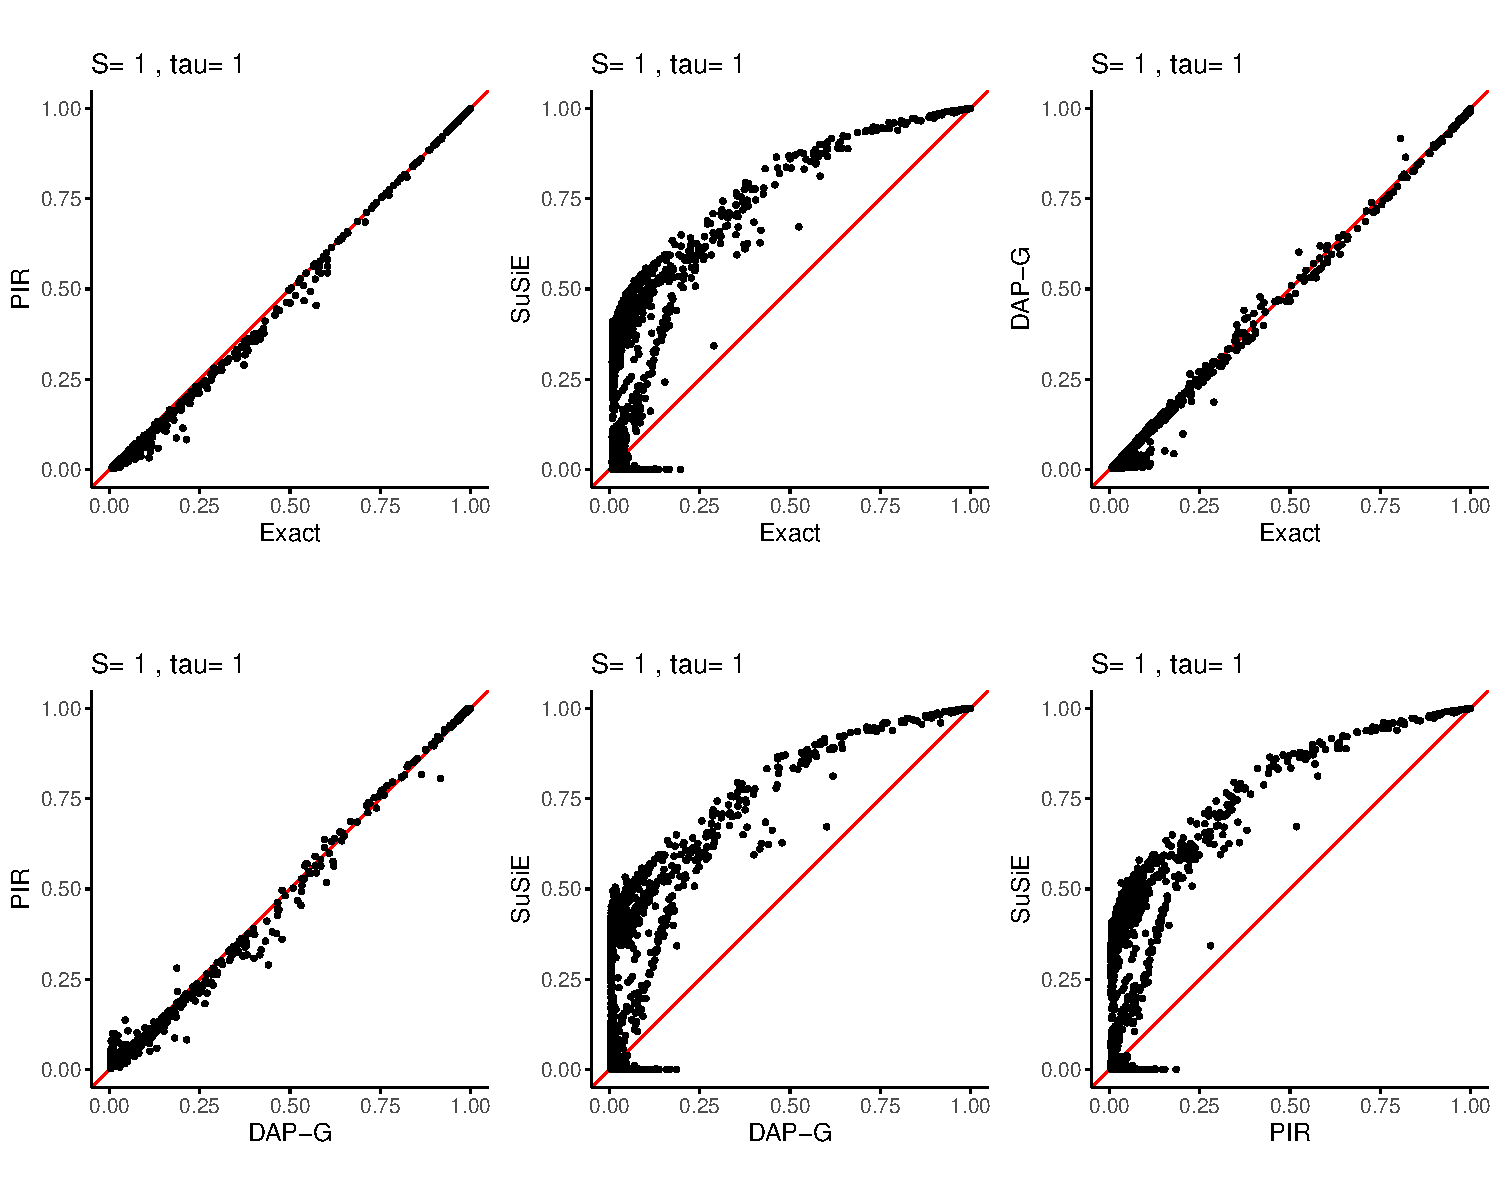
\includegraphics[width=\textwidth, page=1]{files/S1.pdf}
    \caption{PIP calibration plots of DAP-PIR, DAP-G, SuSiE and exact calculation with $S=1$.}
    \label{fig11}
\end{figure}
\begin{figure}[H]
    \centering
    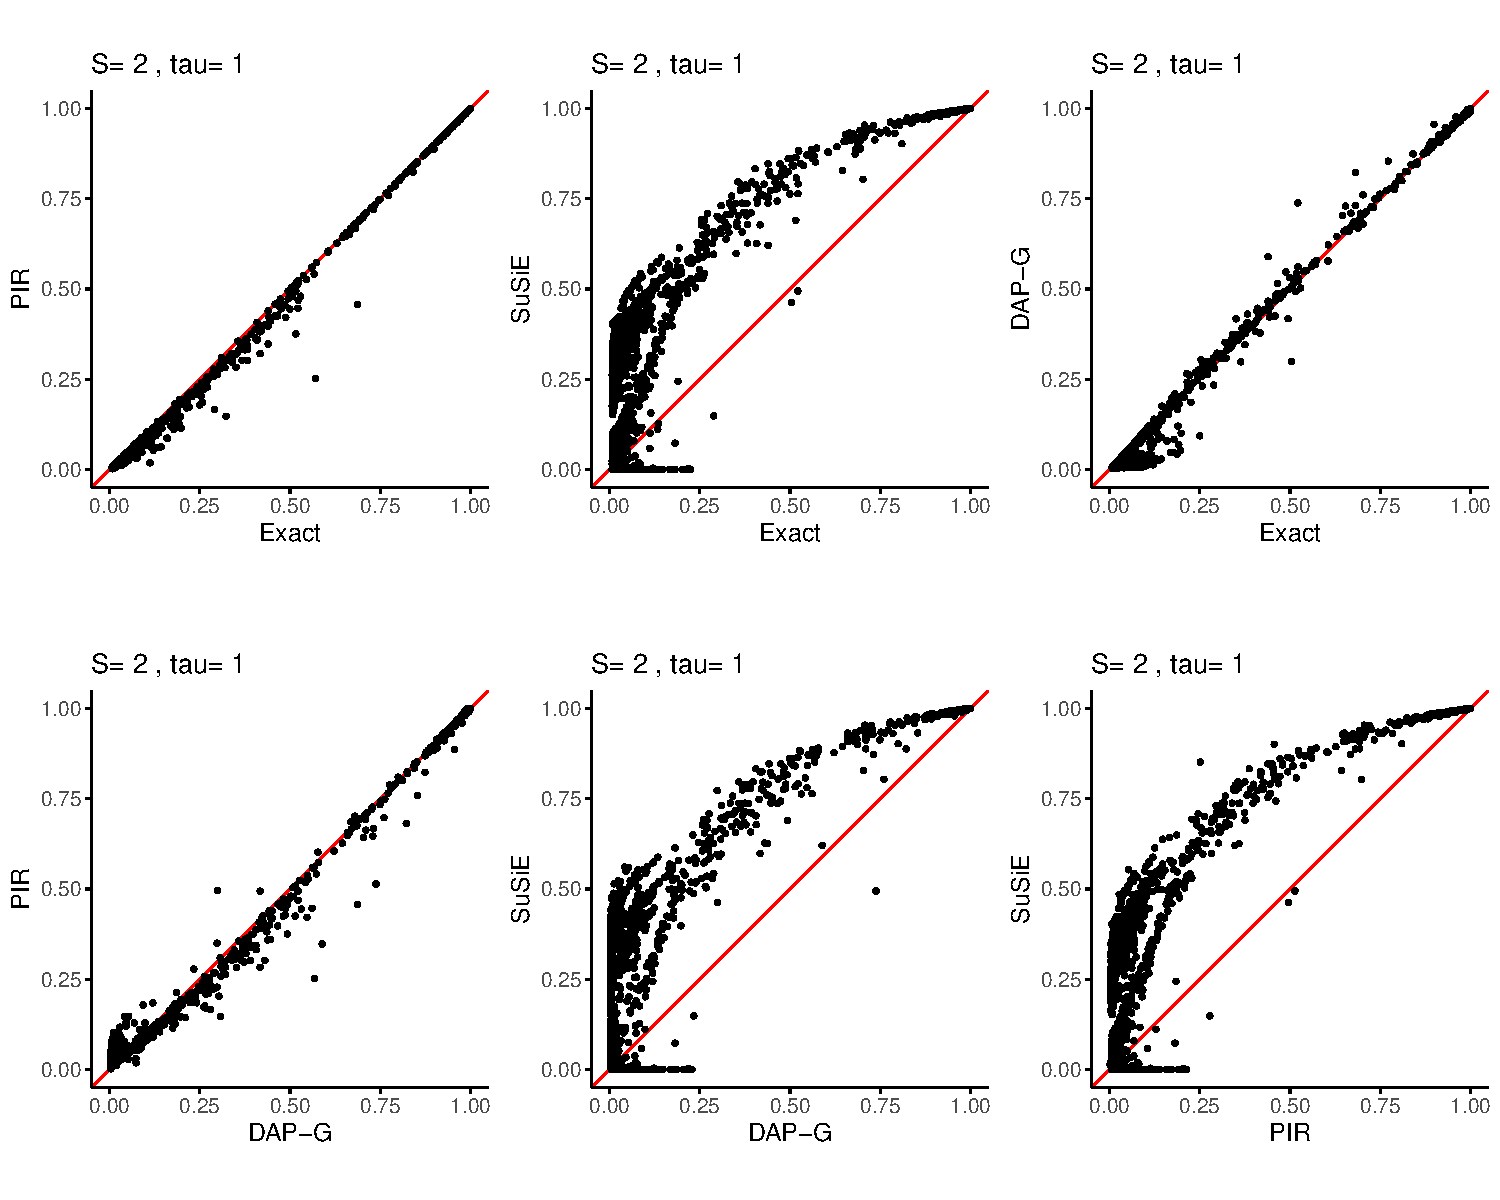
\includegraphics[width=\textwidth, page=1]{files/S2.pdf}
    \caption{PIP calibration plots of DAP-PIR, DAP-G, SuSiE and exact calculation with $S=2$.}
    \label{fig21}
\end{figure}
\begin{figure}[H]
    \centering
    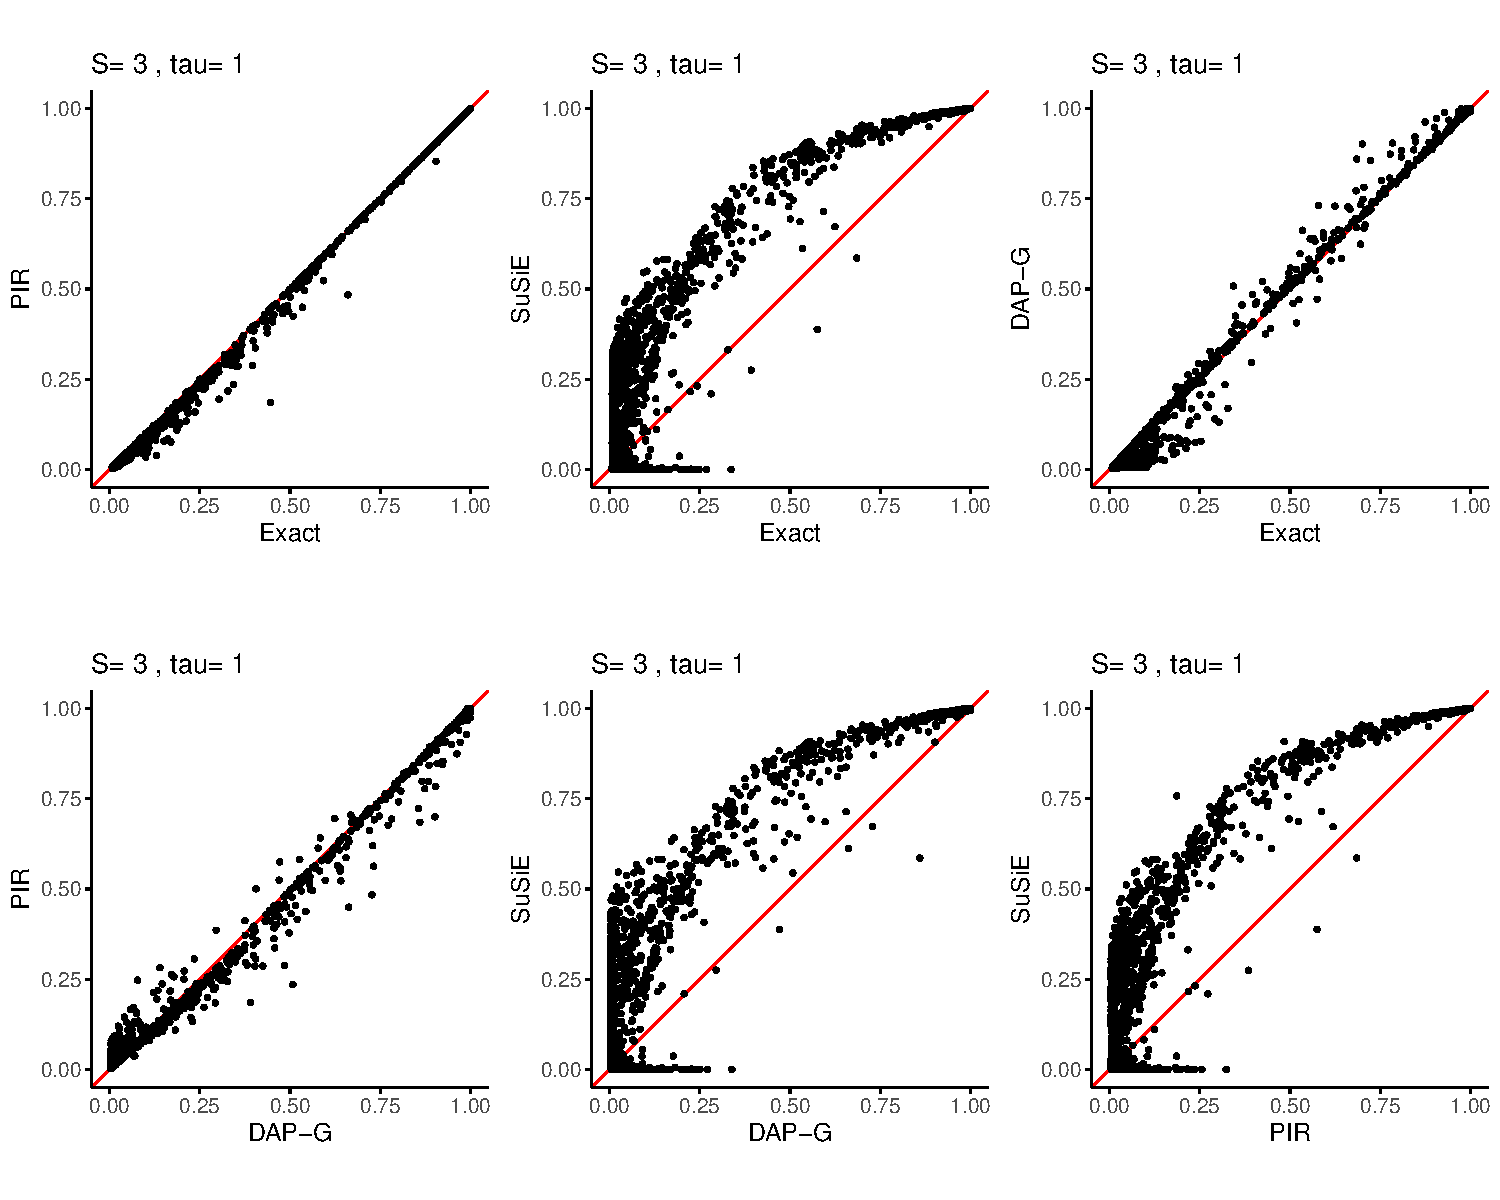
\includegraphics[width=\textwidth, page=1]{files/S3.pdf}
    \caption{PIP calibration plots of DAP-PIR, DAP-G, SuSiE and exact calculation with $S=3$.}
    \label{fig31}
\end{figure}
\begin{figure}[H]
    \centering
    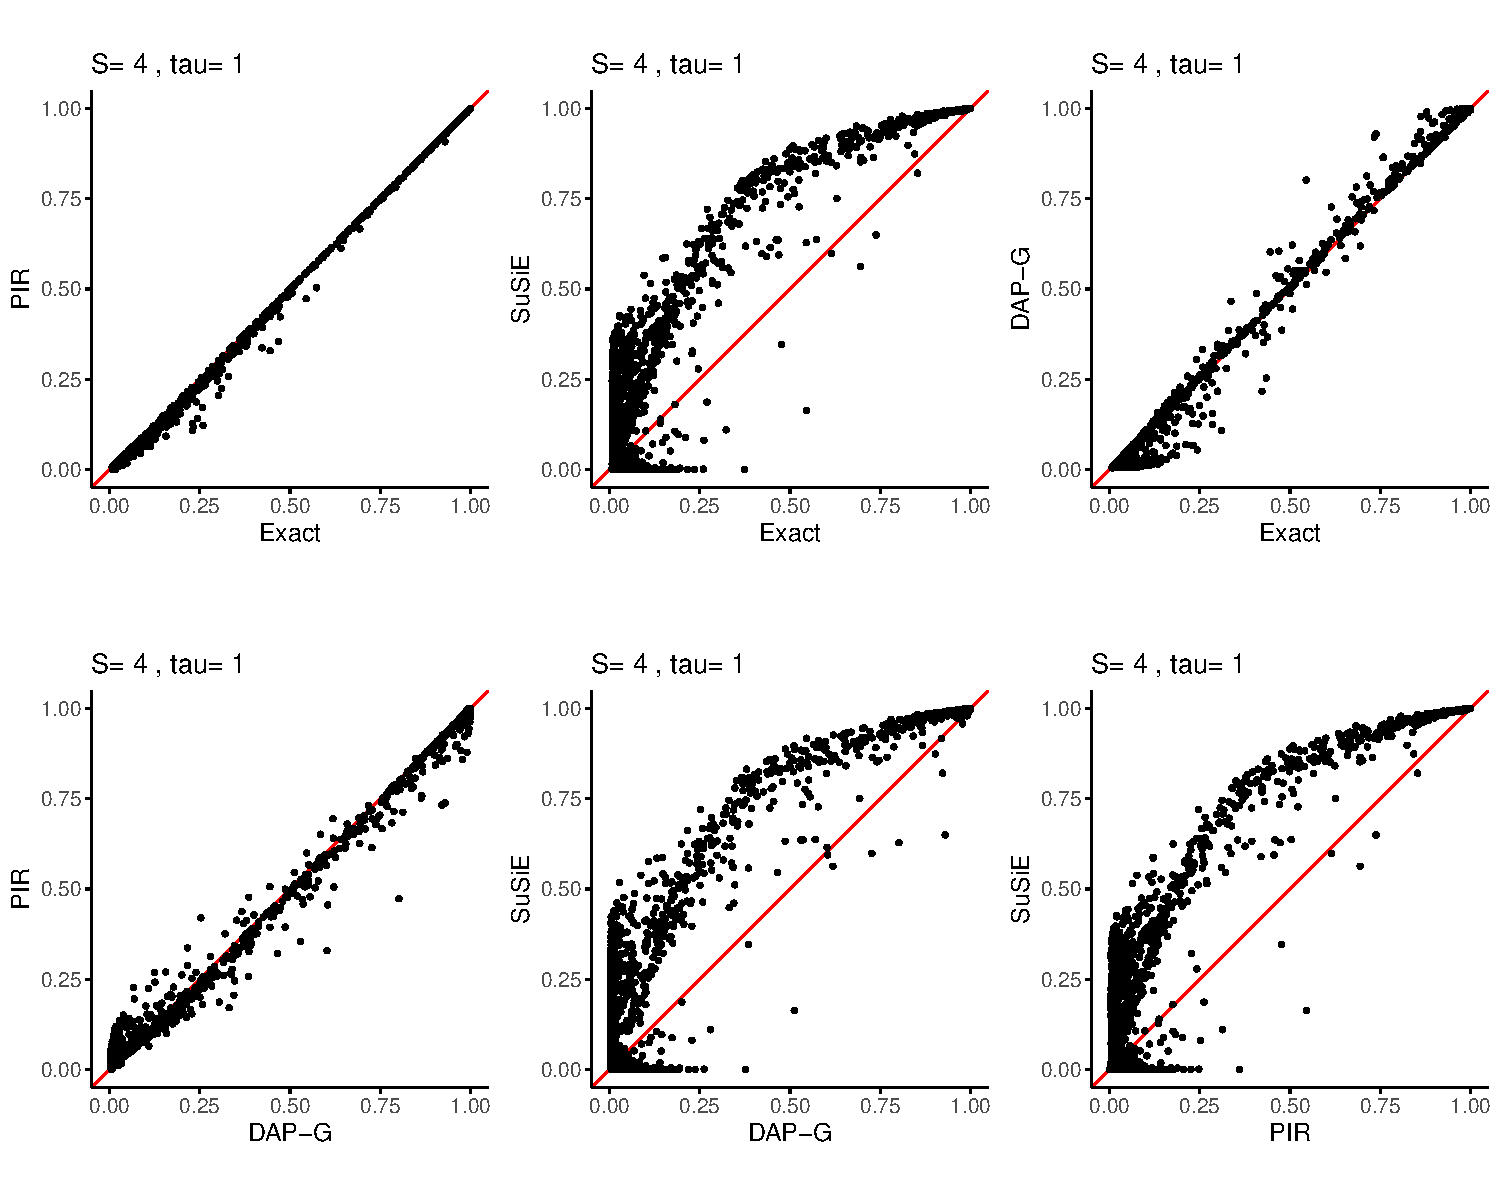
\includegraphics[width=\textwidth, page=1]{files/S4.pdf}
    \caption{PIP calibration plots of DAP-PIR, DAP-G, SuSiE and exact calculation with $S=4$.}
    \label{fig41}
\end{figure}
\begin{figure}[H]
    \centering
    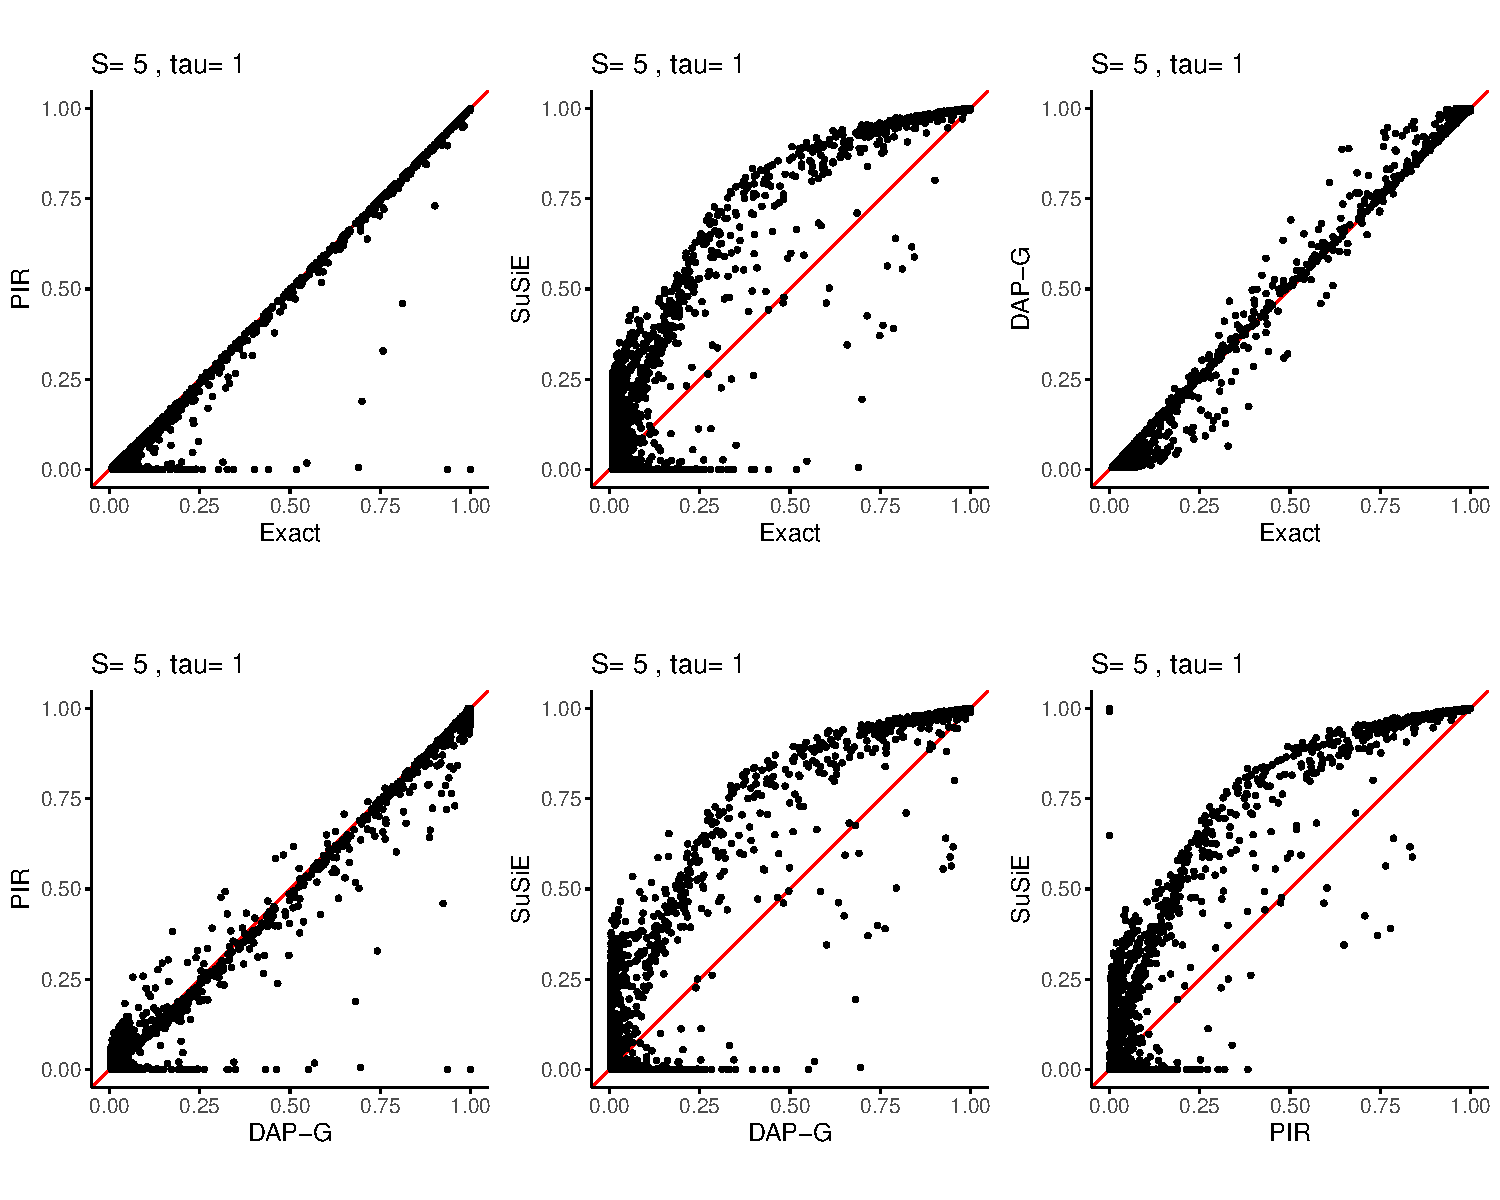
\includegraphics[width=\textwidth, page=1]{files/S5.pdf}
    \caption{PIP calibration plots of DAP-PIR, DAP-G, SuSiE and exact calculation with $S=5$.}
    \label{fig51}
\end{figure}




\newpage
\bibliography{references}

\end{document}
